\section{Design workshop}
\label{sec:designWorkshop}
Before the first sprint, a design workshop was held. Hanne Linander, a
master student in Industrial Design at NTNU was responsible for the workshop.
The goal was to come up with different ideas for functionality and design, and
make an early sketch for the layout of the application.

At this stage in the study, we had not yet decided to develop two separate
applications, so we created layout suggestions for an application aimed to do
both tasks for children and for adults.

Many different exercises were completed throughout the day, in order to make as many
creative ideas as possible. Examples of exercises are short time boxed sketch
sessions, cross-collaboration without explaining thoughts behind the sketches,
different idea-competitions, among others. At the end the ideas were evaluated,
resulting in many discards and some being taken into further development.
After the workshop the sketches and the ideas were presented to the customer.
The development team was very happy about the results and decided to develop a
paperprototype from the sketches.

\subsection{Results}
We drew several sketches of how we envisioned the different views in an 
imagined Android application. 

Figure \ref{fig:dwMainMenu} shows a suggestion for the main menu in the 
application, where the action of taking medicine is in focus. The menu includes:
\begin{itemize}
  \item a log button where an adult can view medication history for the child,
  \item a manual button for learning how to use medication,
  \item a settings button for adjusting mediation schedule, alarm ringtone etc.,
  \item an ``about the app'' button for learning how to use the application,
  \item a display where one can view the current health state for the child, and
  		also click on it to change the health state, and
  \item a count of how many stars the child has collected, with the option to
  		click on that count to see more detailed information about the rewards
  		collected.
\end{itemize}

Figure \ref{fig:dwHealthState} illustrates how a user would see the health state
view separately from the menu. It would consist of three elements represented as
colored smileys; one for each health state. The healthy smiley would be green and
smiling, the sick one would be yellow and in a mellow mood, while the very sick
state would be represented by a red, frowning smiley. The currently active health
state could be displayed by illuminating the respective smiley, and clicking on
another would change the active state.

Figure \ref{fig:dwHealthStatePopup} shows how the health state view could be 
integrated into the main menu better by injecting it into an overlay. This could
make navigating the app more intuitive.

Figure \ref{fig:dwMediationView} is an image of the view a user would first see
when clicking the big ``medicine'' button in the main menu, or the view he or she
sees when redirected from a notification. It shows an image of the medicine to be
taken, and gives the option to go directly to the medication process through
clicking on the medicine image itself. If a user is unsure about how to use the
medication, there is illustrated an option where one would directly be brought to
the manual page for that medicine.

Figure \ref{fig:dwPickChild} shows a view one would be brought to if more than one
child was registered in one application. It shows an icon for each child and the
child's name. Clicking one one or the other would bring the user to the distraction
page for that child.

Figure \ref{fig:dwMediationViewCloudsThunderstorm} is an image of the first part of
the distraction animation a child would see. It shows dark clouds and a thunderstorm
that represents the child's state before taking medication. It was thought of as a 
way to motivate children to take medication in order to clear up the clouds, and as
something children could relate to by comparing their progress to the clouds.

Figure \ref{fig:dwMediationViewEmergingMedicine} is also part of the distraction
animation. It shows a medicine unit emerging from behind the clouds which are clearing
up while the medication is ongoing. The emerging medication was supposed to symbolize
the goodness of medication, while the clearing of clouds would symbolize the child's
lungs and airways clearing up.

Figure \ref{fig:dwChildRewardsView} illustrates how a child could view his or her
collected stars. There is a big star with a count next to it, which would show the 
total amount of stars. In addition, there is a scrolling view on the top where each
day would have an amount of stars on it, corresponding to how many stars the child had
received on that day. Lastly, there is an appealing figure on the page, in this case
a ``ninja master'', which would be an avatar for the child. It was imagined as
something that the child would purchase or obtain after reaching a certain amount of stars,
and the object itself would vary, serving as an additional motivational factor to
supplement the stars themselves.

Figure \ref{fig:dwAdultLogView} is a view where adults could check the progress and
medication history for a child. It would display graphs of condition and how good they
were at following a medication plan. Days would be colored after what condition the 
child was in on that day. The amount of stars the child collected is also shown in each
day, and a percentage of how often a given medicine is taken on the planned time is
displayed on the bottom right.

\begin{figure}
	\begin{minipage}[b]{0.46\linewidth}
		\centering
			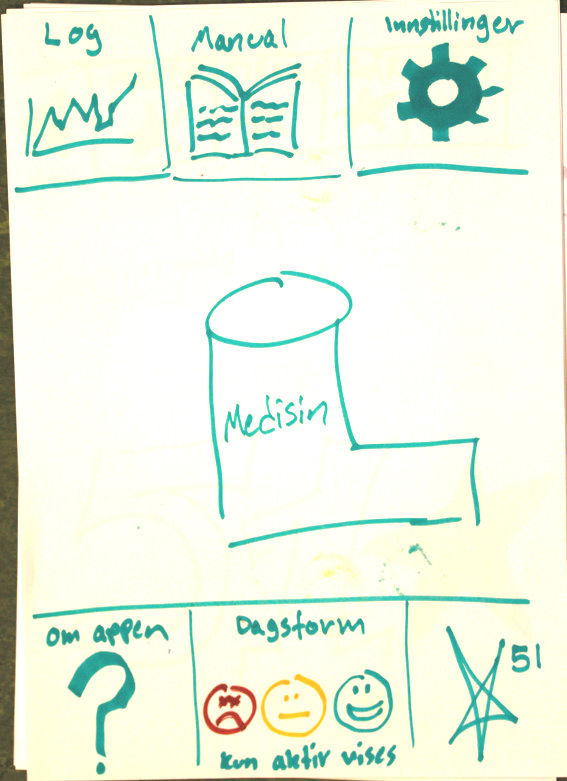
\includegraphics[width=0.34\paperwidth]{Pictures/DesignWorkshop/MobileMainMenu}
		\caption[Main menu view from design workshop]{View for the main menu of the application.}
		\label{fig:dwMainMenu}
	\end{minipage}
	\hspace{1cm}
	\begin{minipage}[b]{0.46\linewidth}
		\centering
		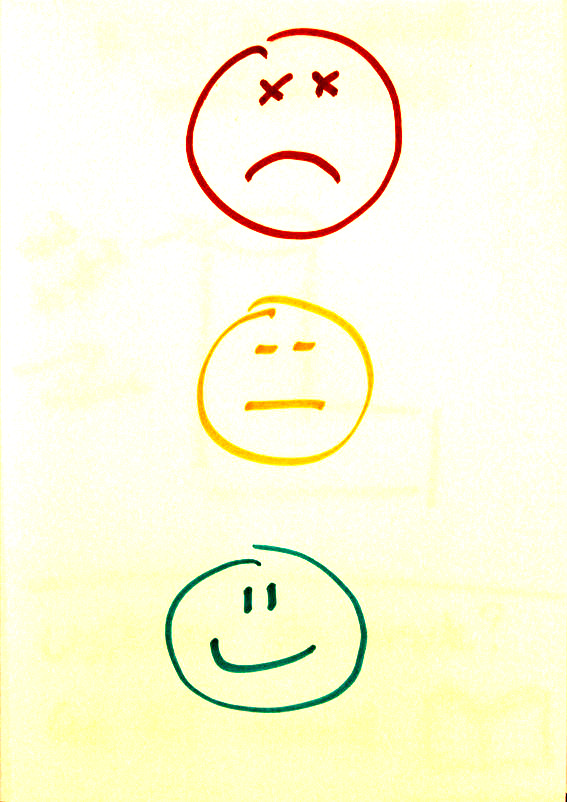
\includegraphics[width=0.34\paperwidth]{Pictures/DesignWorkshop/HealthStateView}
	\caption[Change health state view from design workshop]{View for changing health state (active medication plan).}
	\label{fig:dwHealthState}
	\end{minipage}
\end{figure}

% \begin{figure}
% 	\begin{center}
% 		\includegraphics[width=7cm]{}
% 		\caption{View for the main menu of the application.}
% 		\label{fig:dwMainMenu}
% 	\end{center}
% \end{figure}

% \begin{figure}
% 	\begin{center}
% 		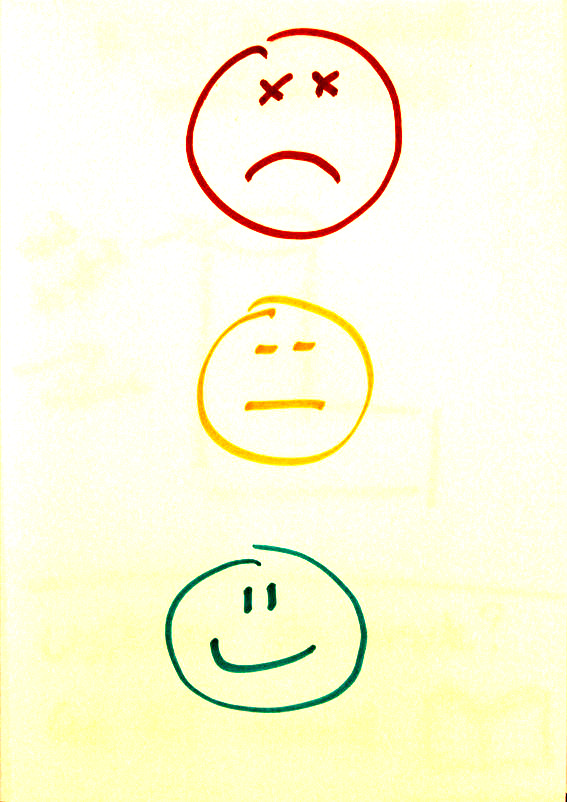
\includegraphics[width=7cm]{Pictures/DesignWorkshop/HealthStateView}
% 		\caption{View for changing health state (active medication plan).}
% 		\label{fig:dwHealthState}
% 	\end{center}
% \end{figure}

\begin{figure}
	\begin{minipage}[b]{0.46\linewidth}
		\centering
			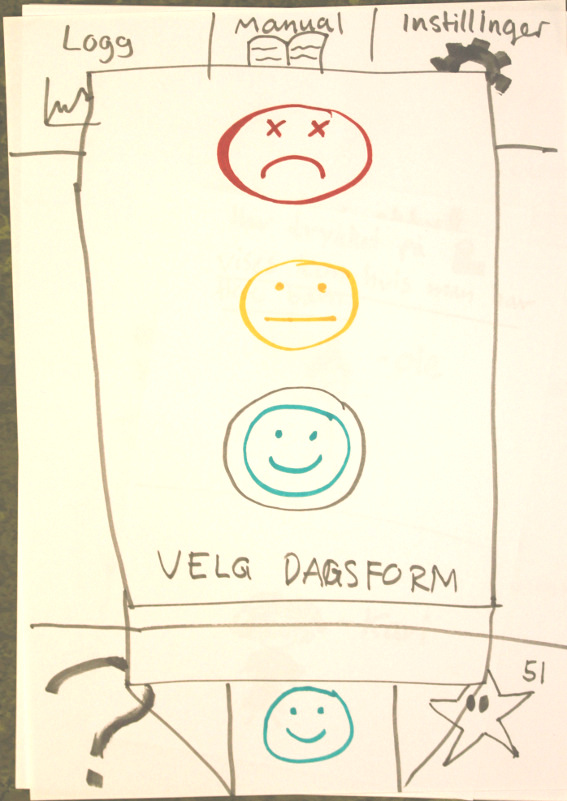
\includegraphics[width=0.34\paperwidth]{Pictures/DesignWorkshop/HealthStateViewPopup}
		\caption[Change health state as pop up from design workshop]{View for changing health state as a pop up from the main menu.}
		\label{fig:dwHealthStatePopup}
	\end{minipage}
	\hspace{1cm}
	\begin{minipage}[b]{0.46\linewidth}
		\centering
		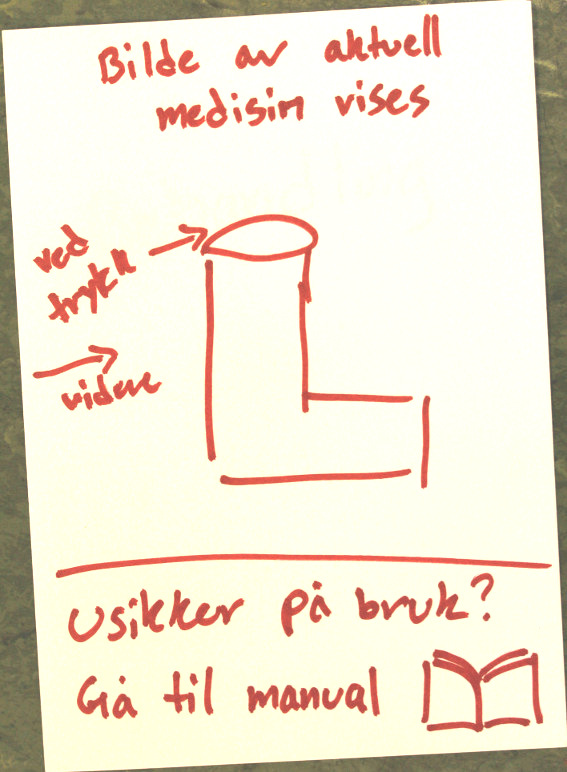
\includegraphics[width=0.34\paperwidth]{Pictures/DesignWorkshop/MedicationView}
	\caption[Start medication view from design workshop]{View for starting a medication and distraction process.}
	\label{fig:dwMediationView}
	\end{minipage}
\end{figure}

% \begin{figure}
% 	\begin{center}
% 		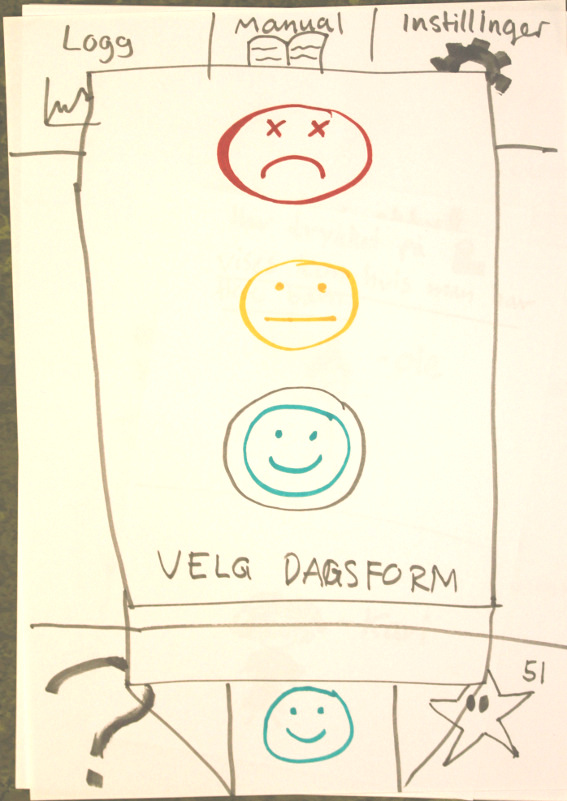
\includegraphics[width=7cm]{Pictures/DesignWorkshop/HealthStateViewPopup}
% 		\caption{View for changing health state as a popup from the main menu.}
% 		\label{fig:dwHealthStatePopup}
% 	\end{center}
% \end{figure}
% 
% \begin{figure}
% 	\begin{center}
% 		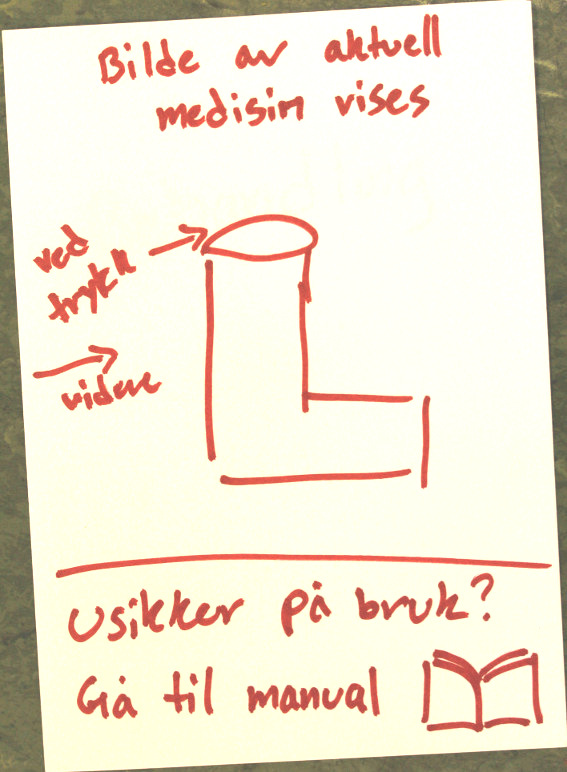
\includegraphics[width=7cm]{Pictures/DesignWorkshop/MedicationView}
% 		\caption{View for starting a medication and distraction process.}
% 		\label{fig:dwMediationView}
% 	\end{center}
% \end{figure}

\begin{figure}
	\begin{minipage}[b]{0.46\linewidth}
		\centering
			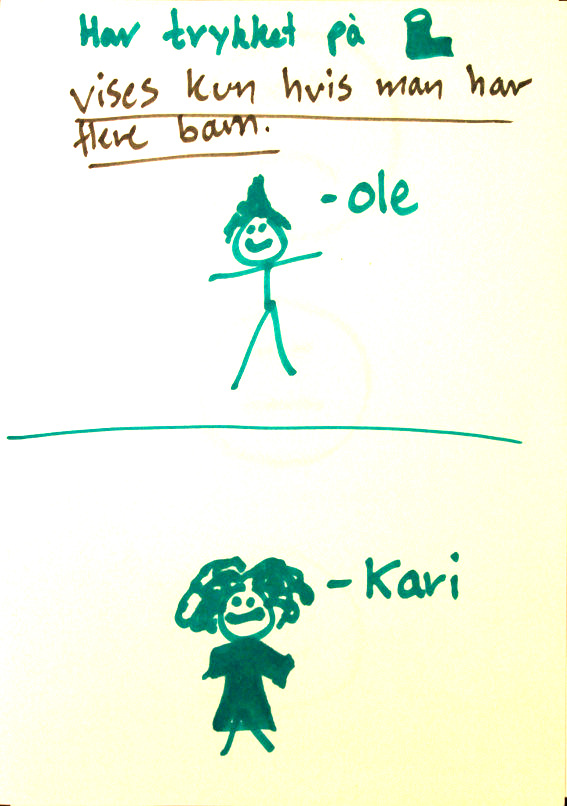
\includegraphics[width=0.34\paperwidth]{Pictures/DesignWorkshop/MedicationViewPickChild}
		\caption[Pick child view from design workshop]{View for choosing child to medicate at the start of medication mode.}
		\label{fig:dwPickChild}
	\end{minipage}
	\hspace{1cm}
	\begin{minipage}[b]{0.46\linewidth}
		\centering
		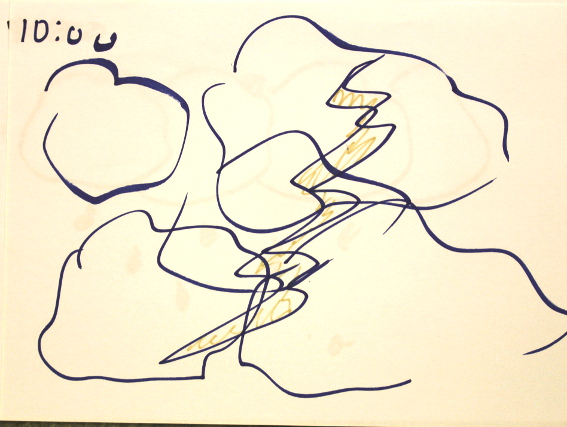
\includegraphics[width=0.34\paperwidth]{Pictures/DesignWorkshop/MedicationViewCloudsThunderstorm}
	\caption[Distraction view from design workshop]{Initial view of a distraction. Heavy clouds and thunderstorms represent the child's state before taking medicine.}
	\label{fig:dwMediationViewCloudsThunderstorm}
	\end{minipage}
\end{figure}

% \begin{figure}
% 	\begin{center}
% 		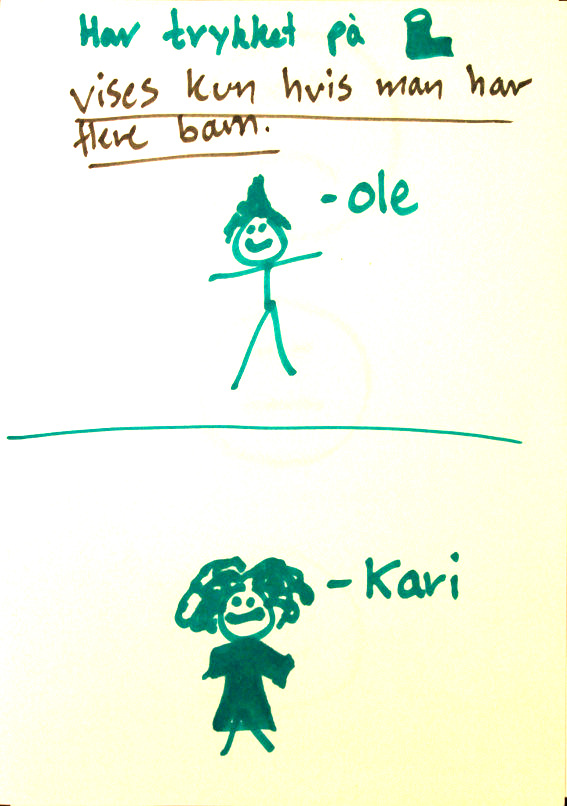
\includegraphics[width=7cm]{Pictures/DesignWorkshop/MedicationViewPickChild}
% 		\caption{View for choosing child to medicate at the start of medication mode.}
% 		\label{fig:dwPickChild}
% 	\end{center}
% \end{figure}
% 
% \begin{figure}
% 	\begin{center}
% 		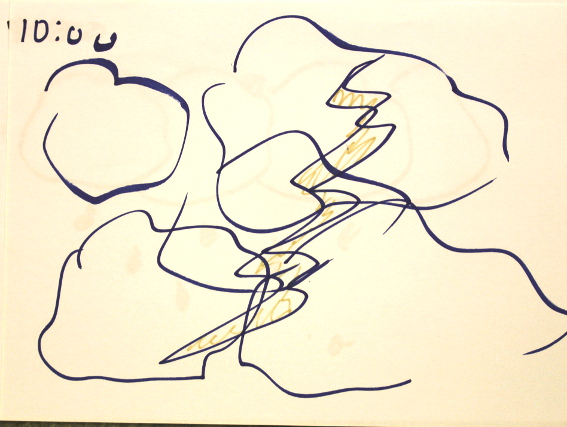
\includegraphics[width=7cm]{Pictures/DesignWorkshop/MedicationViewCloudsThunderstorm}
% 		\caption{Initial view of a distraction. Heavy clouds and thunderstorms represent the child's state before taking medicine.}
% 		\label{fig:dwMediationViewCloudsThunderstorm}
% 	\end{center}
% \end{figure}

\begin{figure}
	\begin{minipage}[b]{0.46\linewidth}
		\centering
			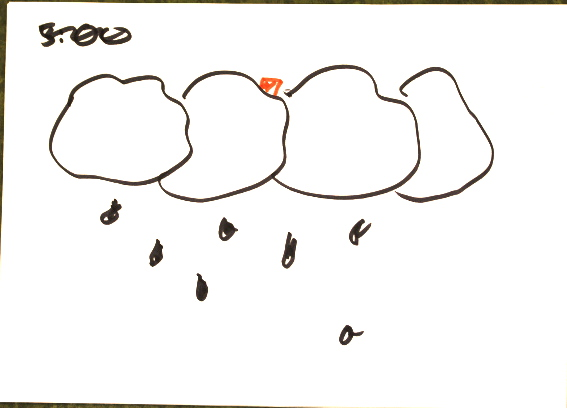
\includegraphics[width=0.34\paperwidth]{Pictures/DesignWorkshop/MedicationViewEmergingMedicine}
		\caption[Distraction view 2 from design workshop]{Subsequent view of a distraction process. The medication is emerging while the clouds are disappearing, to symbolize the healing effects of medicine.}
		\label{fig:dwMediationViewEmergingMedicine}
	\end{minipage}
	\hspace{1cm}
	\begin{minipage}[b]{0.46\linewidth}
		\centering
		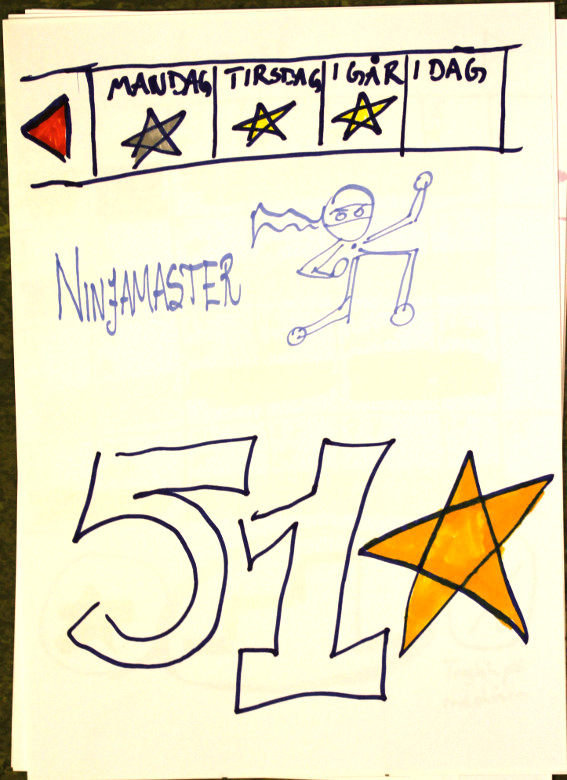
\includegraphics[width=0.34\paperwidth]{Pictures/DesignWorkshop/ChildRewardsView}
	\caption[Rewards view from design workshop]{View where children can view their collected reward (stars), and an acquired rank (in this case ``ninja master'').}
	\label{fig:dwChildRewardsView}
	\end{minipage}
\end{figure}

% \begin{figure}
% 	\begin{center}
% 		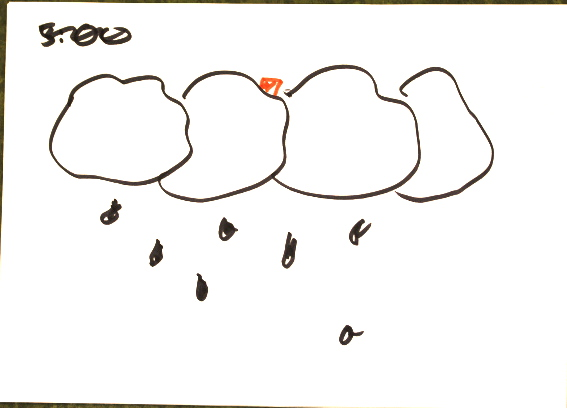
\includegraphics[width=7cm]{Pictures/DesignWorkshop/MedicationViewEmergingMedicine}
% 		\caption{Subsequent view of a distraction process. The medication is emergin while the clouds are disapeparing, to symbolize the healing effects of medicine.}
% 		\label{fig:dwMediationViewEmergingMedicine}
% 	\end{center}
% \end{figure}
% 
% \begin{figure}
% 	\begin{center}
% 		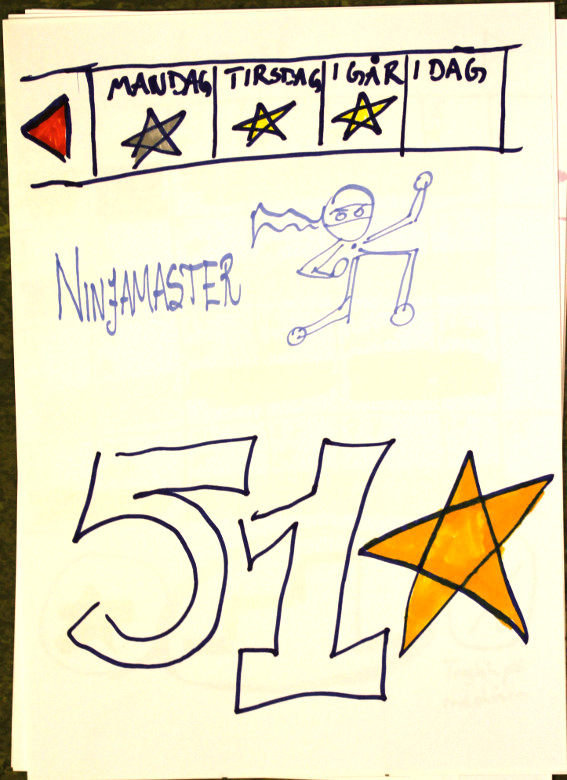
\includegraphics[width=7cm]{Pictures/DesignWorkshop/ChildRewardsView}
% 		\caption{View where children can view their collected reward (stars), and an acquired rank (in this case ``ninja master'').}
% 		\label{fig:dwChildRewardsView}
% 	\end{center}
% \end{figure}

\begin{figure}
	\begin{center}
		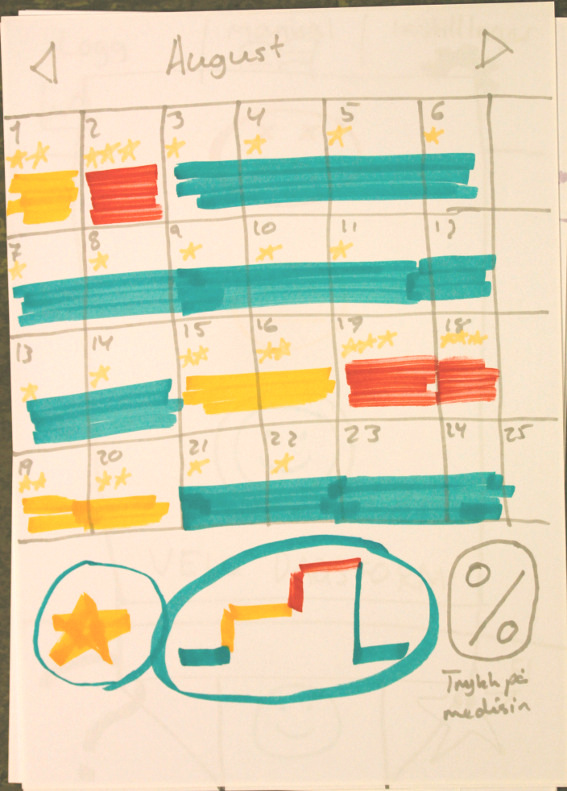
\includegraphics[width=7cm]{Pictures/DesignWorkshop/AdultLogView}
		\caption[Log view from design workshop]{View where adults can view the medication and health state history for a child.}
		\label{fig:dwAdultLogView}
	\end{center}
\end{figure}
\clearpage{}
\subsection{What was used in the further development}
Several ideas from the design workshop was used later in the development. We realized that we did not have sufficient time to make a very complicated distraction and
reward system for CAPP, so we decided to keep the ideas from the workshop about rewarding the child with stars whenever he or she completed a treatment.
This is easily implementable, and we believed it would be easy for parents to build on it with physical rewards when the child had accumulated enough stars.
For the same reasons we chose to keep and build on the idea of having an animation sequence where a Karotz avatar mirrored what the child had to do, it would
equip the inhalation mask when the child had to, making it more exciting for the child to do this as well. This approach have been seen to work with other applications,
like for helping children brush their teeth, and we wanted to use this as our base point.

We did the workshop based on the idea of having
one application, but later decided on having two. This meant that most of the basic GUI elements we came up with here, had
to be redone. For GAPP we implemented a log which kept its general layout, with the coloring showing which plan had been followed the relevant day. We later switched around on the additional information
that would be shown on each date and how, but the concept stayed the same.